%!TEX root = ../diplom.tex

\section{Моделирование процесса измерения}



При малых углах падения механизм обратного  рассеяния является квазизеркальным
и отражение происходит на участках волнового профиля, ориентированных
перпендикулярно падающему излучению. Тогда в формировании отраженного сигнала
будут участвовать только площадки, ориентированные нормально к излучению. 
Поэтому для моделирования рассеяния нам необходимо знать не только высоту в
точке, но и уравнение касательной к ней плоскости, для этого необходимо знать
наклоны $\zeta_x$ и  $\zeta_y$ в искомой точке
\footnote{Под словосочетанием <<отражающая точка>> подразумевается физически
бесконечно малая площадка, характерные размеры  которой больше длины волны
радиолокатора}. 

Зная координаты радиолокатора  $(x_{rad},y_{rad},H_0)$, координаты точки на
поверхности $(x,y,\zeta)$, можем из геометрии (см. рис. \ref{fig:local_theta})

\begin{equation}
    \label{eq:local_theta}
    \cos \theta = \frac
    {\zeta_x (x - x_{rad}) + \zeta_y (y - y_{rad}) - (\zeta - H_0) }
        {
           \sqrt{(x - x_{rad})^2 + (y - y_{rad})^2 + (\zeta - H_0)^2 }
           \sqrt{\zeta_x^2 + \zeta_y^2 + 1}
        }
\end{equation}

Вероятность того, что угол $\theta$ будет точно равен нулю и произойдет
зеркальное отражение для случайной выбранной точки очень мала, поэтому имеет
смысл рассматривать квазизеркальное отражение и вводить ограничение на
максимально допустимый локальный угол отражения. 

Нахождение всех зеркальных точек на характерном пятне радиолокатора  $> 1
\text{ км}^2$ представляет собой ресурсоемкую задачу. Но поскольку формирование
импульса носит статистический характер, то мы может выбирать гораздо меньшую
выборку зеркальных точек. 

Процесс создания такой выборки продемонстрирован на рис. \ref{fig:mirror:a}-\ref{fig:mirror:c}. 

Для смоделированной поверхности  рис. \ref{fig:mirror:a} для некоторой
выборки точек вычисляются по формуле \eqref{eq:local_theta} локальные углы
падения. Квазизеркальными позже считаются те, для которых угол меньше одного
градуса $\theta < 1^\circ$. Выборку можно делать несколькими способами,
например создать её выбирая случайные точки на координатной сетке или проходить
координатную сетку с равномерным шагом. 
Выборка на рис. \ref{fig:mirror:b} и \ref{fig:mirror:c} получена вторым
способом. 

\begin{figure}[h!]
    \centering
    \includesvg{local_theta}
    \caption{Геометрия определения локального угла падения. Красной линией
    обозначена касательная плоскость к рассматриваемой отражающей точке
$(x,y,\zeta)$}
    \label{fig:local_theta}
\end{figure}

\begin{figure}[h]
    \centering
    \begin{subfigure}{0.65\linewidth}
        \centering
        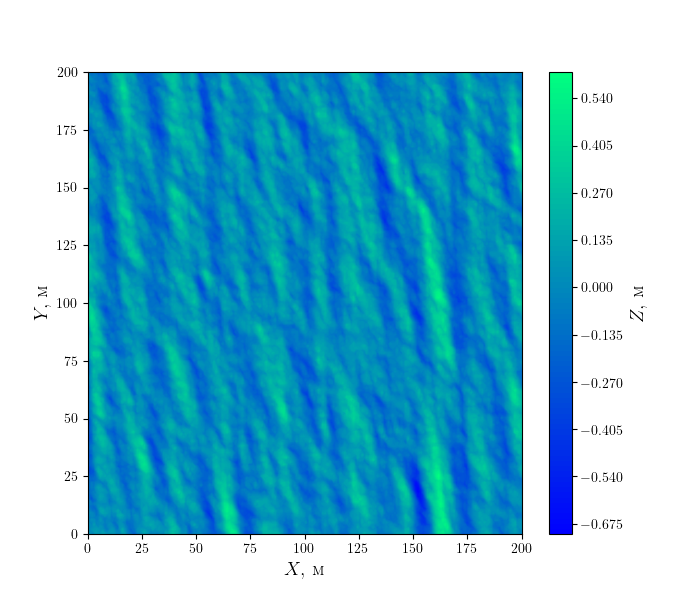
\includegraphics[width=\linewidth]{fig/impulse/fig1}
        \caption{Моделирование поверхности при скорости ветра $U=5$ м/с}
        \label{fig:mirror:a}
    \end{subfigure}
    \begin{subfigure}{.49\linewidth}
        \centering
        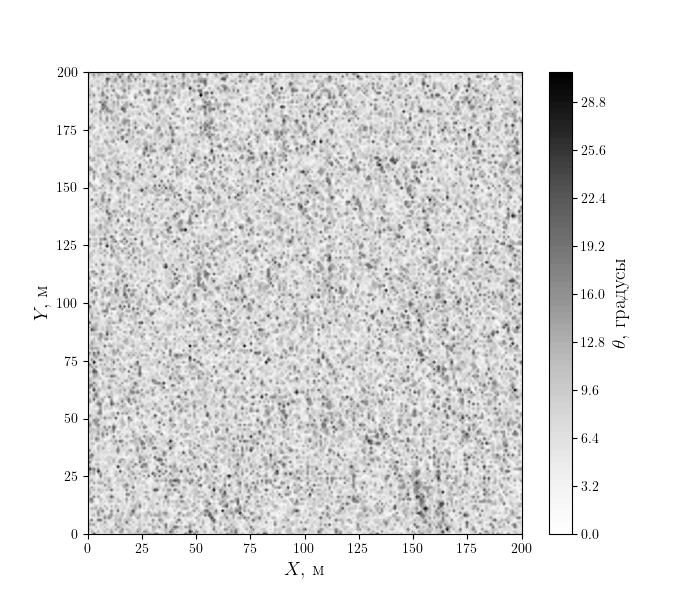
\includegraphics[width=\linewidth]{fig/impulse/fig2}
        \caption{Локальный угол отражения от поверхности для радиолокатора
        находящегося на высоте $H=1000$ км в точке с координатой (100, 100)}
        \label{fig:mirror:b}
    \end{subfigure}
    \begin{subfigure}{.49\linewidth}
        \centering
        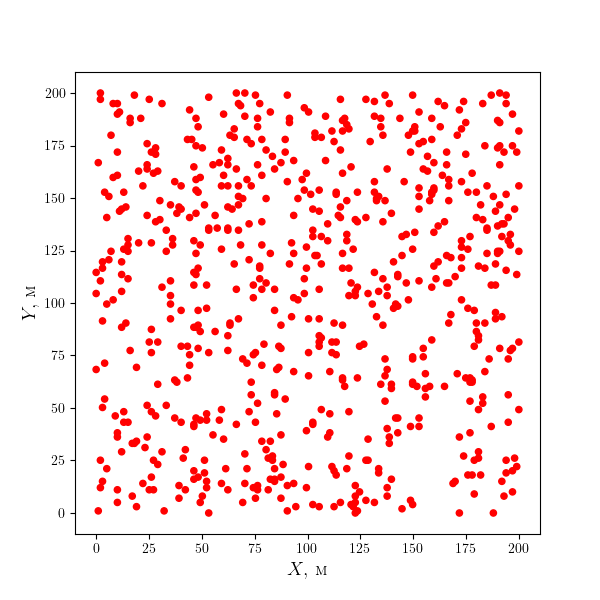
\includegraphics[width=\linewidth]{fig/impulse/fig3}
        \caption{Положение зеркальных точек поверхности \ref{fig:mirror:a} для
        радиолокатора находящегося над точкой (100,100) }
        \label{fig:mirror:c}
    \end{subfigure}
    \label{fig:mirror}
    \caption{}
\end{figure}

Теперь, для вычисления поля вблизи приемной антенны радиолокатора нам
необходимо просуммировать отраженное от квазизеркальных точек поле
(см.рис. \ref{fig:mirror:c}).  


Как было сказано с предыдущих разделах, амплитуда поля излученного антенной
спадает по гиперболическому закону. Тогда амплитуда поля вблизи точки отражения
$(x,y,\zeta)$
будет определяться как (см. геометрию задачи на рис. \ref{fig:local_theta})
\begin{equation}
    \label{eq:}
    E_{sur} \sim \frac{E_0}{R_1} e^{-ikR_1} \cdot G(x,y,\theta_0), 
\end{equation}
Следовательно, вблизи приемной антенны амплитуду можно записать как
\begin{equation}
    \label{eq:E}
    E \sim \frac{E_{sur}}{R_1} e^{-ikR_1} \cdot G(x,y,\theta_0) =
    \frac{E_0}{R_1^2} e^{-2ikR_1} \cdot G^2(x,y,\theta_0), 
\end{equation}

Остается только проинтегрировать уравнение \eqref{eq:E} по всем отражающим
точкам 
\begin{equation}
    \label{eq:}
    E \sim \sum\limits_{i=1}^{M} \frac{E_0}{R_i^2} \exp{-2ikR_i}
    G^2(x,y,\theta_0)
\end{equation}
где $M$ -- количество точек,  $x_i,y_i$ -- координаты  $i-$ой отражающей точки,
 $R_i$-- расстояние от спутника до  $i-$ой точки.
